\section{Speech Emotion Recognition}
Another key element of Pookie’s AI is the Speech Emotion Recognition (SER) system, which is used for recognizing the user’s emotions based on vocal patterns. By analyzing factors such as pitch, tone, and intensity, the system detects emotions: neutral, anger, happiness, sadness, and frustration. This section outlines the current progress, challenges, and future approaches for designing the speech emotion recognition model, including relevant datasets and methodologies.
\subsection{Uvicorn Server}
Significant progress has been achieved in the backend infrastructure development with the successful implementation of the Uvicorn server. The server now effectively facilitates HTTP-based communication with the Speech Emotion Recognition (SER) model. This implementation has notably enhanced our testing capabilities by enabling real-time inference processing.

\begin{figure}[ht]
    \centering
    \captionsetup{justification=centering}
    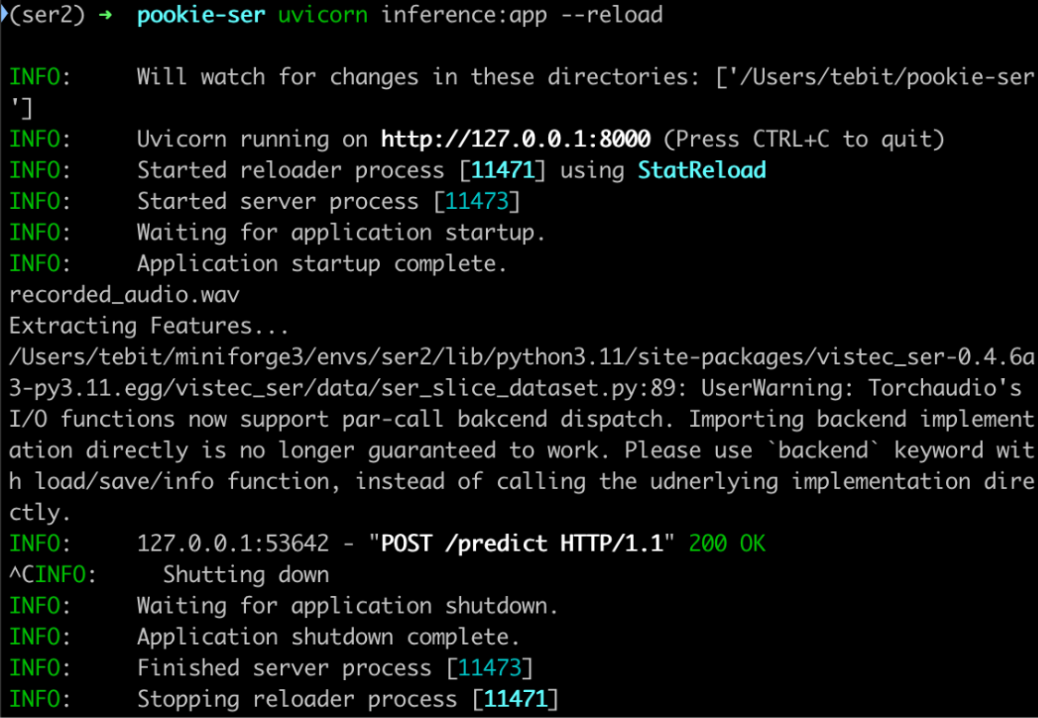
\includegraphics[width=0.8\textwidth]{server.png}
    \caption{Local Uvicorn Server}
    \label{fig:server}
\end{figure}

\newpage
\subsection{Simple Client}
A simple client application has been successfully developed with the implementation of essential functionalities. The terminal-based interface allows users to control audio recording durations through keyboard inputs. The client manages the workflow from audio capture to server communication, handling the transmission of recorded files and displaying emotion recognition results as they are processed.

\begin{figure}[ht]
    \centering
    \captionsetup{justification=centering}
    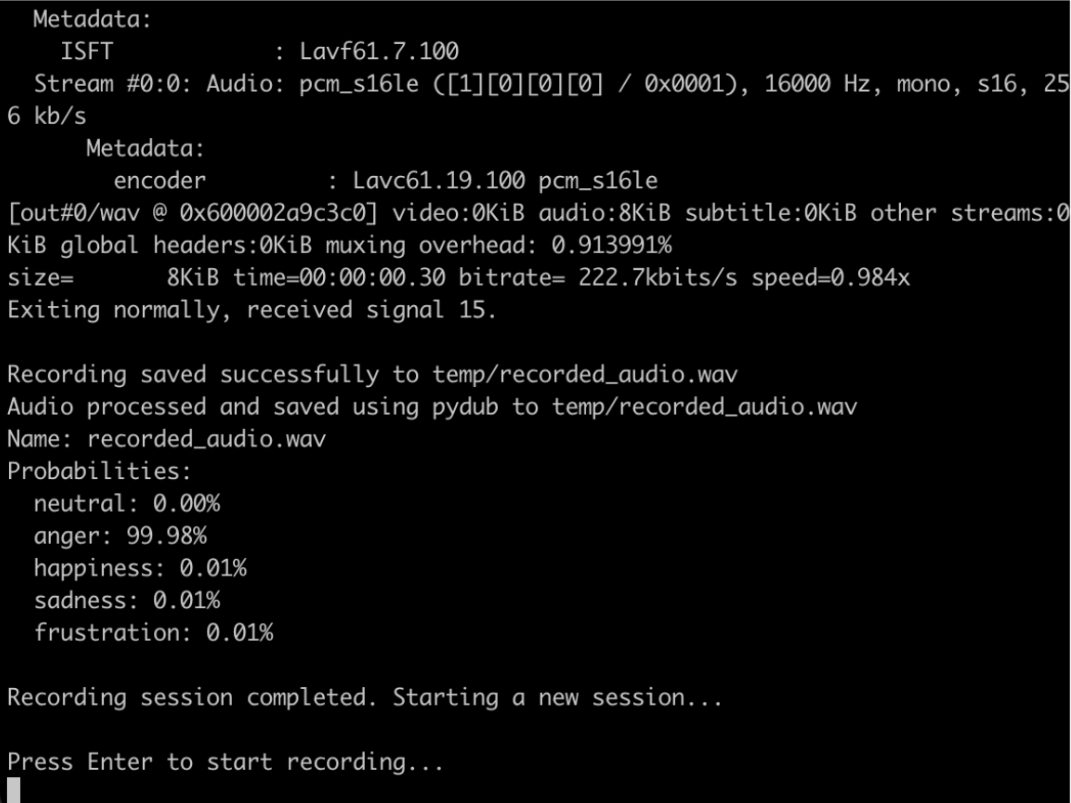
\includegraphics[width=0.8\textwidth]{client.png}
    \caption{Simple Client}
    \label{fig:client}
\end{figure}

\newpage
\subsection{Results}
Performance testing of the SER model has yielded mixed results. While the system demonstrates exceptional computational efficiency, achieving inference times between 16ms to 36ms when tested on an M1 MacBook Air, the accuracy of emotion recognition requires further refinement. Initial validation testing, conducted using a sample audio clip from timestamp of a reference emotional speech video, revealed significant discrepancies between expected and actual emotion classifications. The audio segment, which clearly exhibits characteristics of sadness, produced inconsistent recognition results. Several factors may contribute to this performance gap, including the model's training on dramatized voice datasets, variations in team members' vocal characteristics, or potential configuration issues in the local deployment environment. These findings indicate a need for model optimization and further investigation into the impact of different voice characteristics on recognition accuracy.

\begin{figure}[ht]
    \centering
    \captionsetup{justification=centering}
    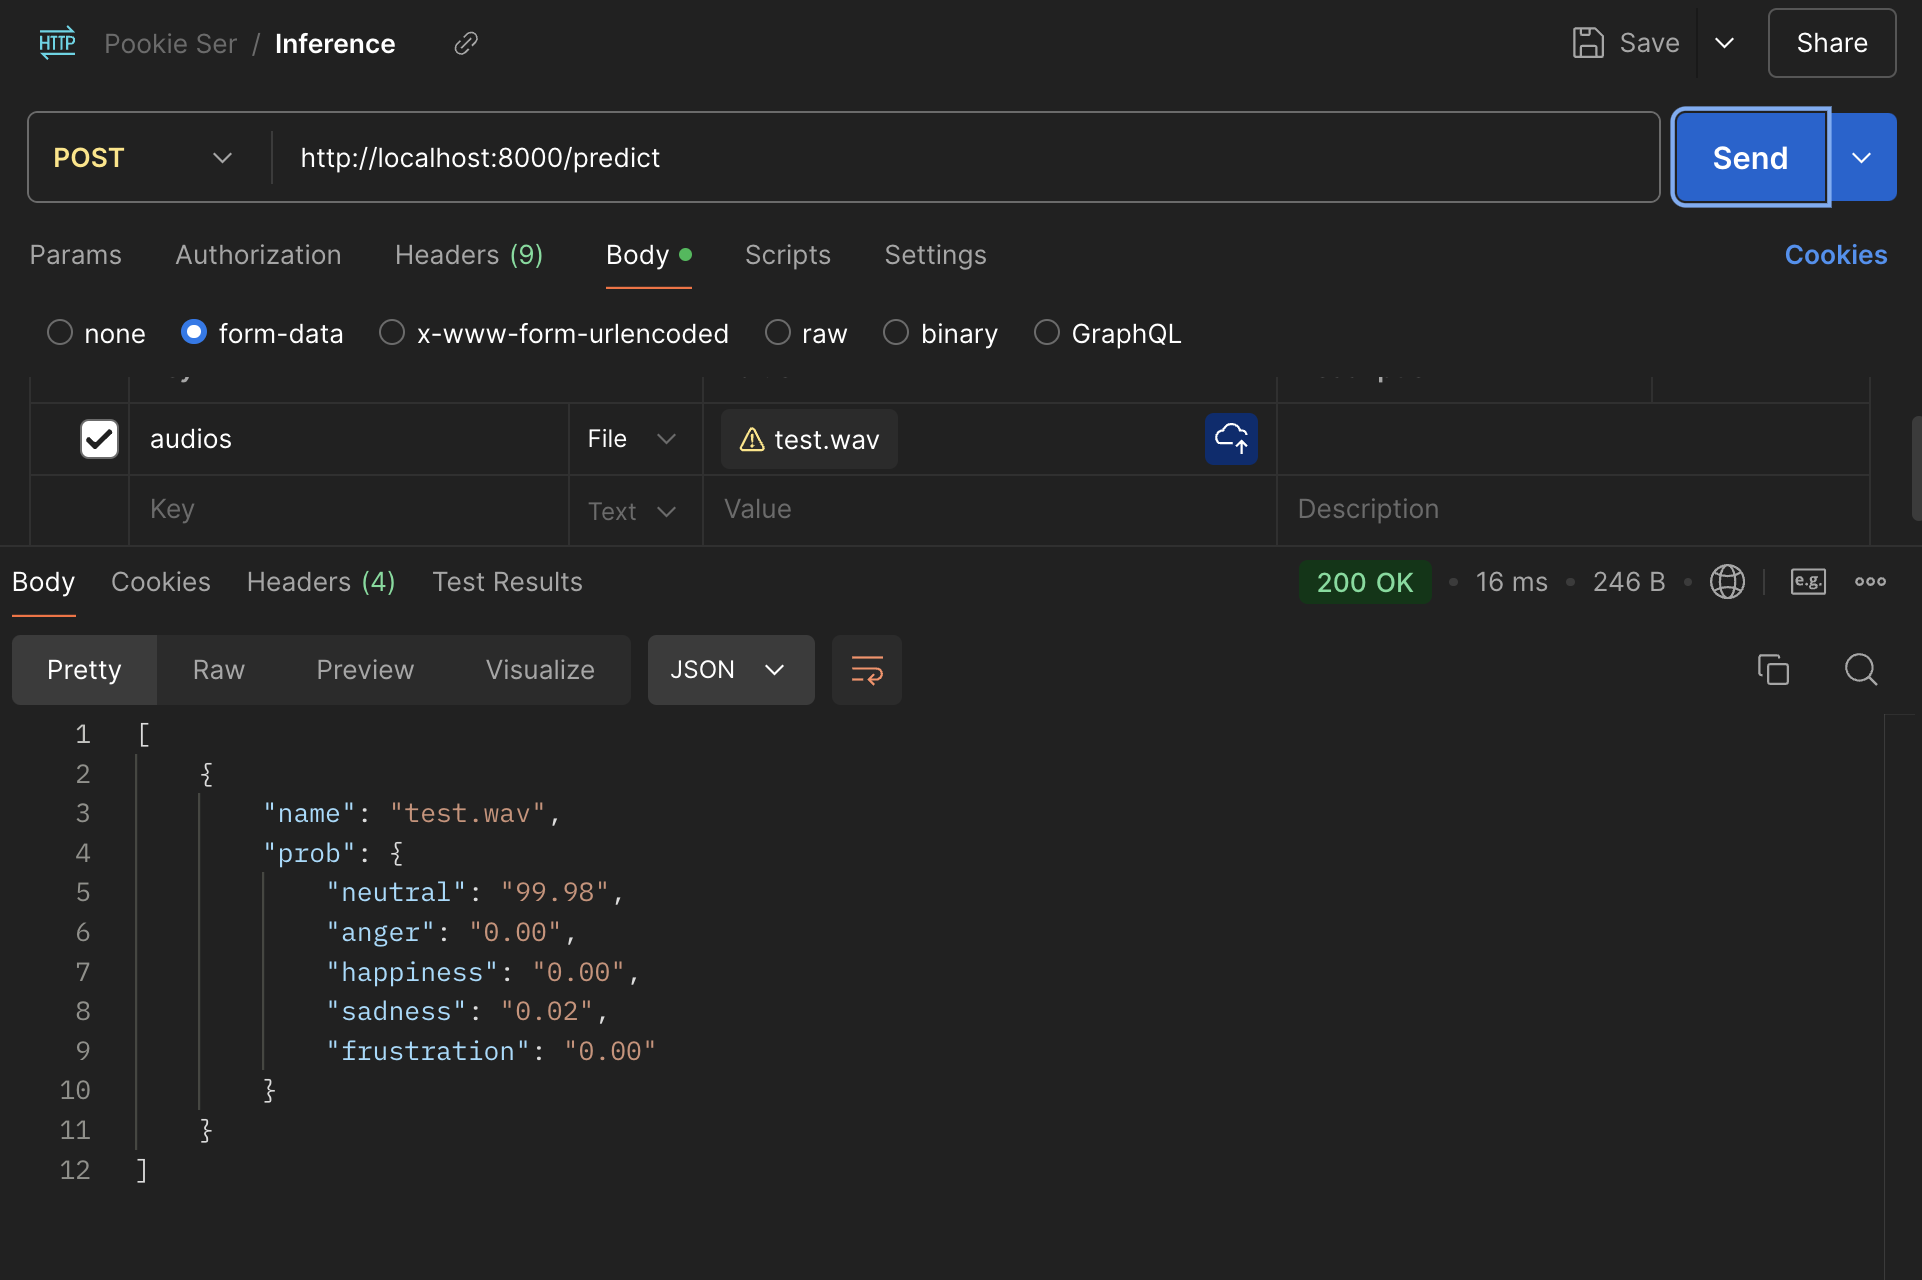
\includegraphics[width=0.8\textwidth]{16ms.png}
    \caption{16ms Inference Time}
    \label{fig:16ms}
\end{figure}

\begin{figure}[ht]
    \centering
    \captionsetup{justification=centering}
    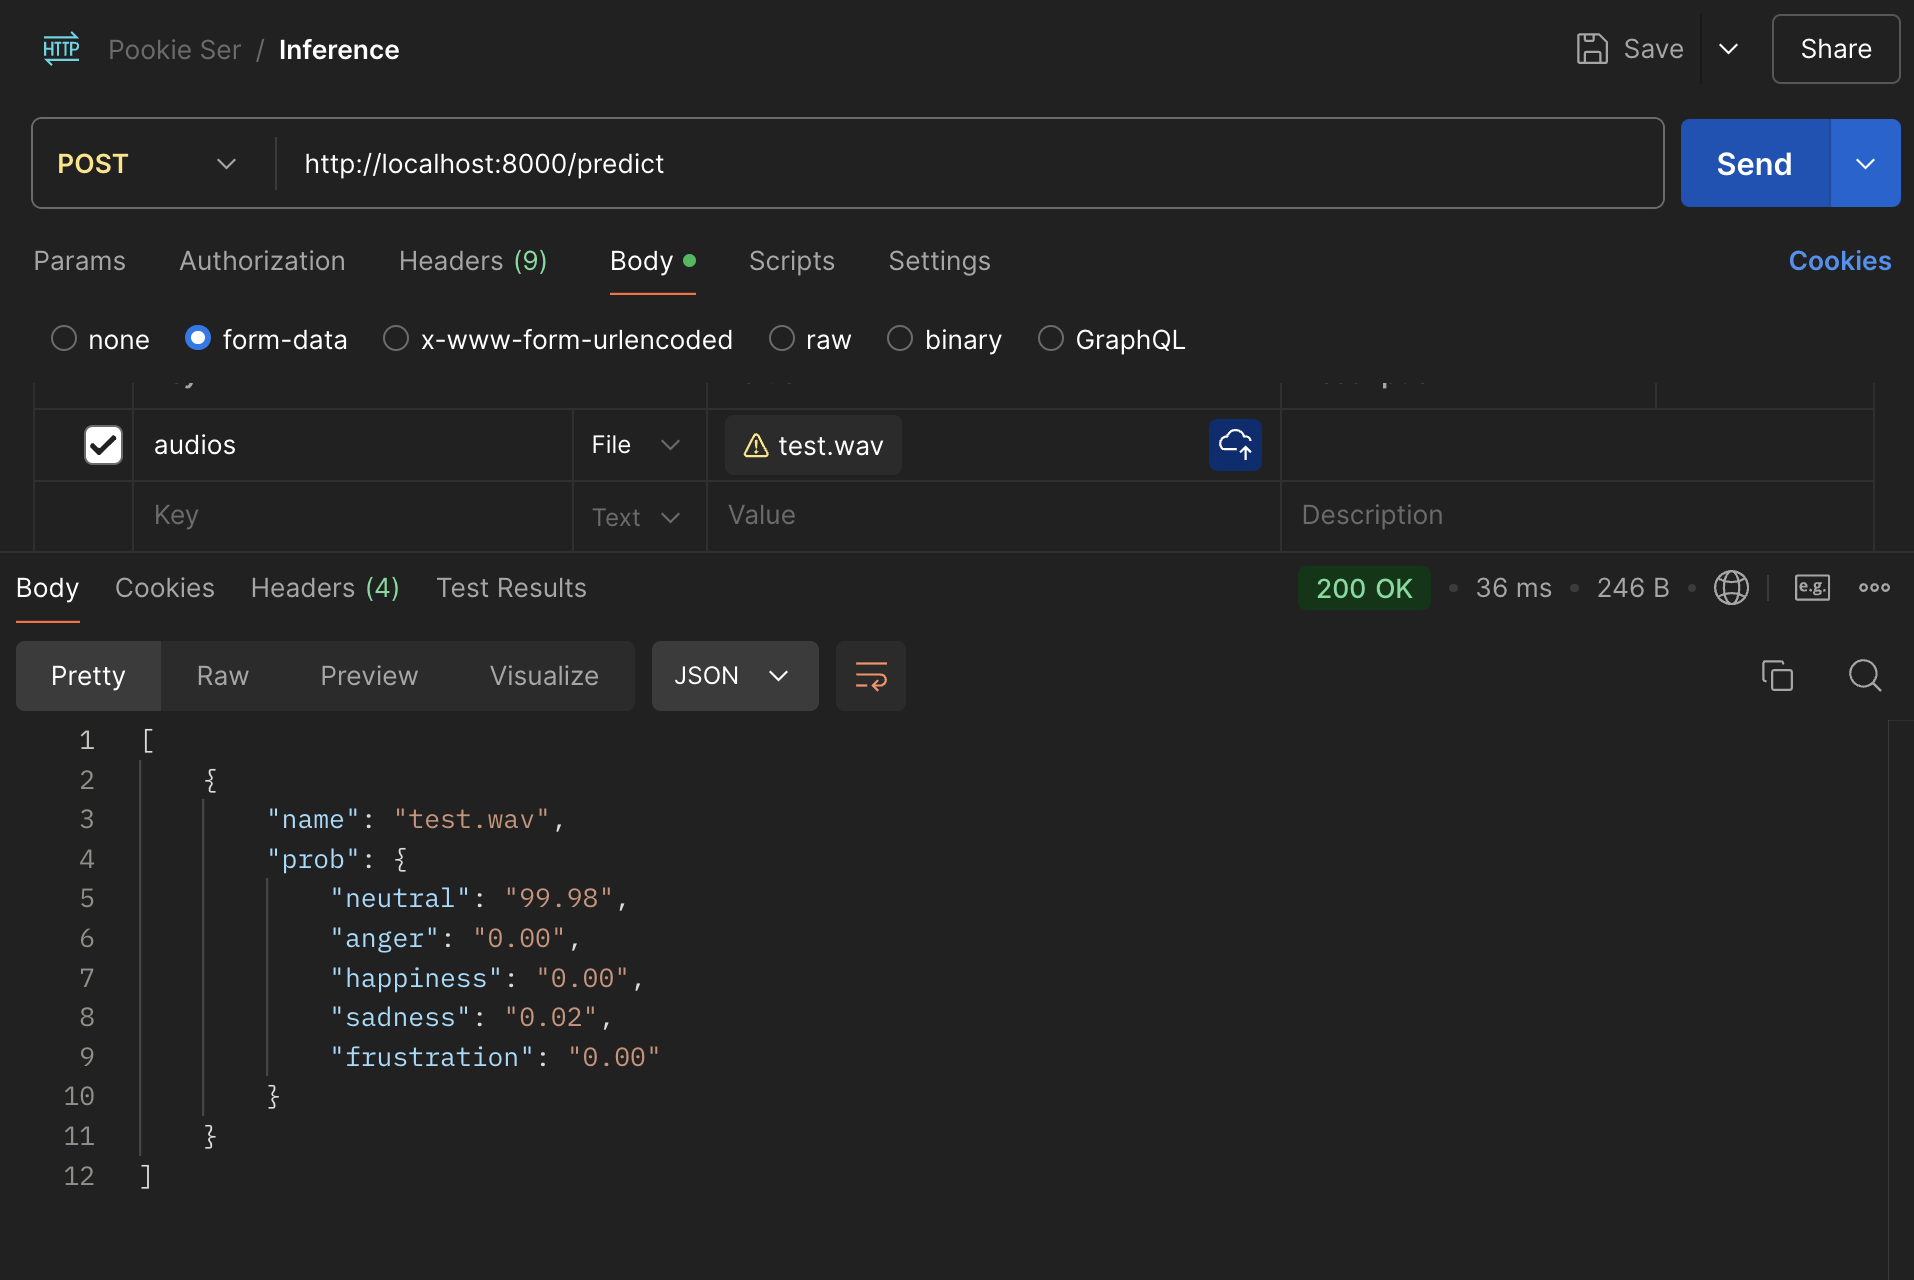
\includegraphics[width=0.8\textwidth]{36ms.png}
    \caption{36ms Inference Time}
    \label{fig:36ms}
\end{figure}

\subsection{Future Actions and Implementation}
The completion of the initial SER system implementation has highlighted several critical areas for future development and optimization. Primary among these objectives is the integration of the Speech Emotion Recognition system with the existing Facial Emotion Recognition (FER) framework through our server infrastructure. Additionally, a comprehensive investigation into the current model's performance discrepancies has been prioritized. This investigation will focus on analyzing the underlying causes of prediction inaccuracies and implementing necessary improvements to enhance the model's reliability. 